\documentclass[12pt]{report}
\usepackage{amsmath}
\usepackage{amssymb}
\usepackage{graphicx}
\usepackage{hyperref}
\usepackage{color}
\usepackage{float}
\begin{document}
	\title{A Model of Histone Sliding with UV Dose Dependency}
	\maketitle
	% setting of the model
	We start with a description of DNA and histone loss from the damage region centered at the origin.
    We set $R_0$ to be the radius of the damage region centered at the UV light's focal point at the origin. Damages to the DNA are considered to spread from the origin to $R_0$ immediately after UVC initiation. We consider a single chromatin strand, initially compacted in the damage region with one end at the origin and the other at $R_0$. We set $n_0$ to be the number of histones on this chromatin strand at time 0.
    
    Post UVC, the chromatin undergoes decompaction until reaching a saturation 15 minutes after. We set $R$ to be the radius to which the damaged chromatin expanded to and consider it as the ROI radius for measurement of DNA and histone loss. With histones assumed to be uniformly distributed before UVC, we have $(R/R_0) n_0$ histones initially in the ROI. 
    
   Chromatin decompaction in the damage region results from the recruitment and crowding of repair protein post UVC to the damage sites. The direction of decompaction is assumed to be from the UVC focal point, for which the concentration of damages is the highest, in a radial manner outwards. As a result of crowding, non-damaged DNA and histones are pushed out of the ROI in equal proportions. 
   
   In addition to the loss by crowding, histones are lost due to sliding away from high concentration of damage site and eventually out of the ROI. Damaged DNA is exposed for repair by repair proteins who slide histones along the chromatin in a general outward radial direction. We set the number of histones remaining on the chromatin strand after saturation to be $n$. Both crowding and sliding of histones expands the damaged region until its saturation at the ROI radius. 
   
   The expansion of the damaged region is measured according to the position of the most exterior damage point on the damaged chromatin strand. Since sliding of a histone over a damage point, displaces this point spatially. 
   By sliding histone over the exterior damage point, the damaged chromatin unpacks and the histone is considered lost. We note that at this point, the length of the damaged chromatin up to the exterior damage point does not change.
        
   Experimental data shows that both histone and DNA loss increase with UV dose. However, the scenario for histone and DNA loss described above is considered to stay similar regardless of the UVC dose. Taking advantage of the radial symmetry in our description, we present a steady-state one-dimensional model of chromatin expansion post UVC and the resulting loss of histone and DNA from the ROI. Let the ratio $n/n_0 =g$, and the expansion factor $R/R_0=\beta$, DNA and histone loss fractions can be represented as function of the UV dose, $u$, by
	\begin{equation}\label{eq:dnaLoss}
	d(u) = \frac{\beta(u)-1}{\beta(u)}
	\end{equation}
	\begin{equation}\label{eq:histoneLoss}
	h(u) = d(u) +\frac{n_0-n(u)}{(R(u)/R_0) n_0}=1-\frac{g(u)}{\beta(u)}
	\end{equation}
 with $0\leq n(u)\leq n_0$, and $u\geq0$. 
 
The fraction of loss by sliding out of the total histone loss is given by
\begin{equation}\label{eq:contributionOfSliding}
\frac{h(u)-d(u)}{h(u)}=\frac{1-g(u)}{\beta(u)-g(u)}
\end{equation}
We estimate this function, by fitting the data to $d(u)$ and $g(u)$. We note that in the UV dose range of 0 to 50, the function $d(u)$ behaves almost linearly. Fitting the data for $d$ we obtain  $d(u)=au$ with $a=0.004$ ($R^2= 0.971$). We 
\begin{figure}[H]
	\centering
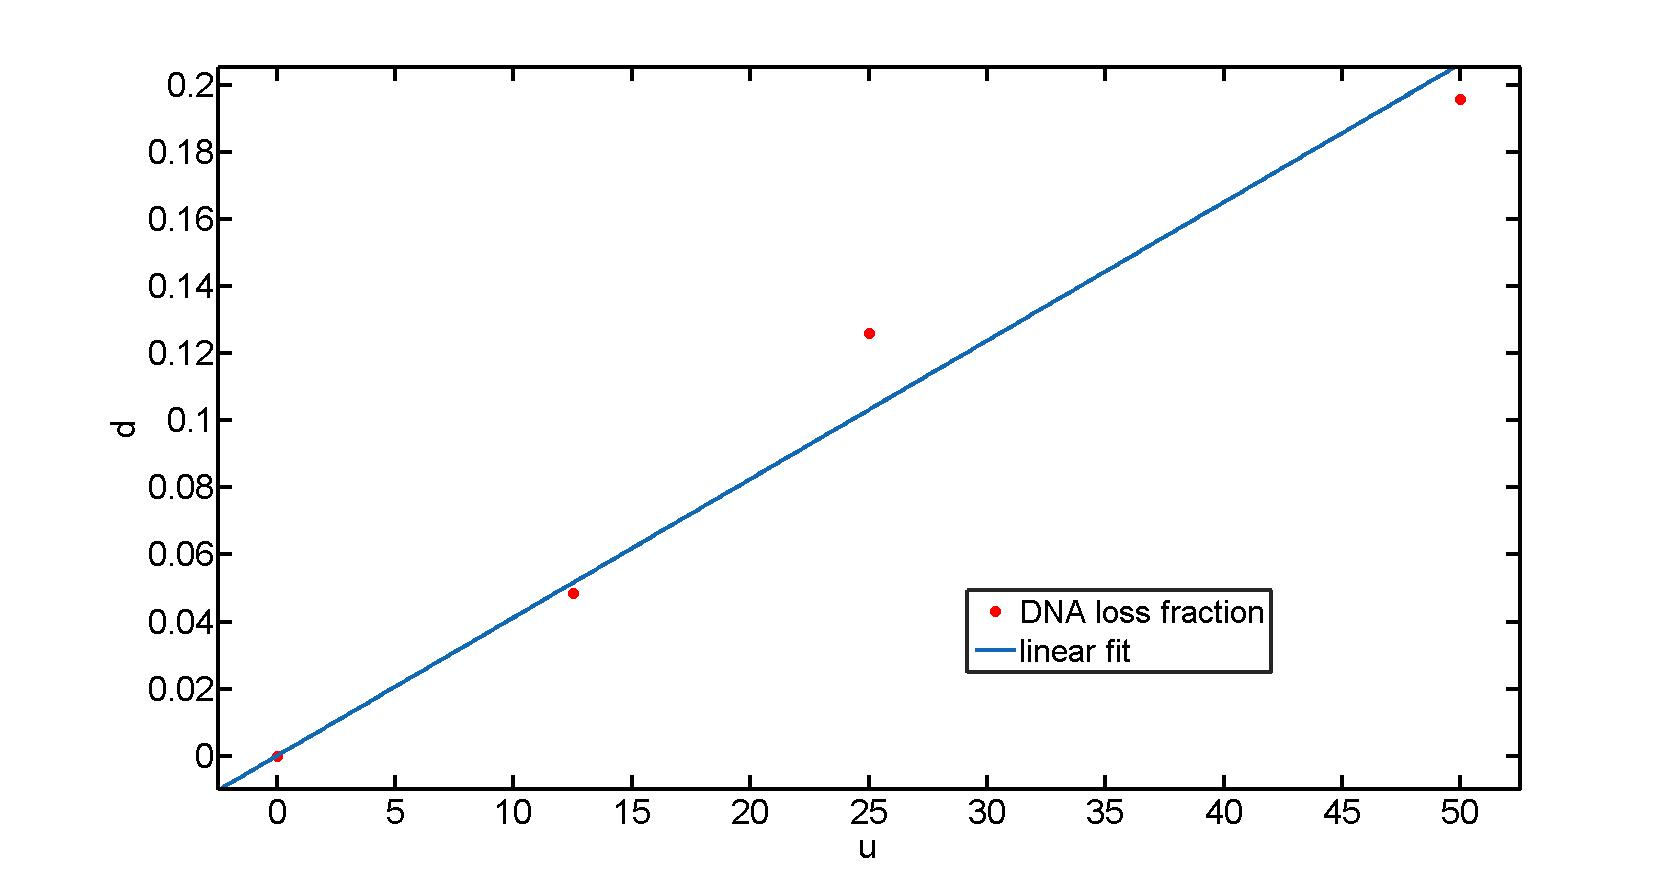
\includegraphics[width=0.5\linewidth, height=0.3\textheight]{Images/dVsUVdoseFitLinear}
\caption{}
\label{fig:dVsUVdoseFitLinear}
\end{figure}
We therefore obtain for $0\leq g \leq 50$
\begin{equation}
\beta(u) = \frac{1}{1-d(u)}=\frac{1}{1-0.004u}
\end{equation} 

To estimate $g(u)$ we note from \ref{eq:dnaLoss}, and \ref{eq:histoneLoss} that 
\begin{equation*}
g(u)=\frac{1-h(u)}{1-d(u)}
\end{equation*}
We find the data for $g(u)$ can be well described using the exponential function $c\exp(-ku) +f$. Taking into account the fact that $g(0)=0$, we can set $f=1-c$ and fit the data. By fitting we find $c=0.185, k=0.044$, ($R^2 =0.981$).

\begin{figure}[H]
	\centering
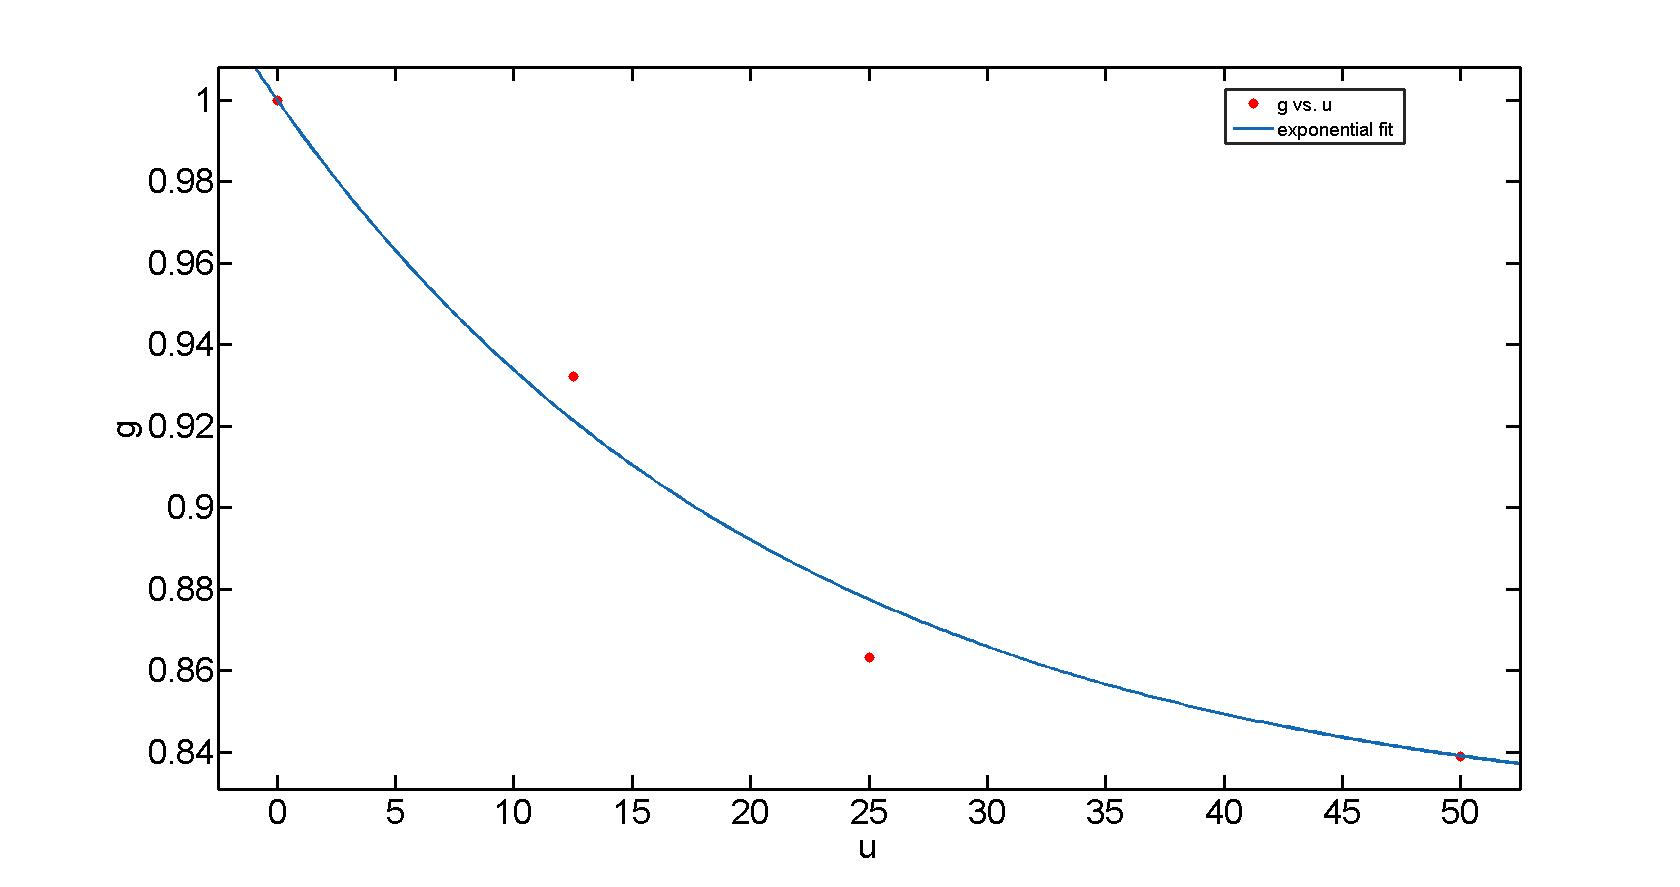
\includegraphics[width=0.5\linewidth, height=0.3\textheight]{Images/gVsUVdoseFitExponential}
\caption{}
\label{fig:gVsUVdoseFitExponential}
\end{figure}

The contribution of sliding to the total histone loss in eq \ref{eq:contributionOfSliding}, can now be given as 
\begin{equation}
\frac{h-d}{h} =\frac{1-g(u)}{\beta(u)-g(u)}= \frac{0.185(1-\exp(-0.044u))}{\frac{1}{1-0.004u}-(1-0.185(1-\exp(-0.044u))}
\end{equation}
A graph of this function is given for values of $u$ between 0 and 50. In the range of UV dose, the decrease in the sliding fraction out of the total histone loss is found to be nearly linear. We discard values of this function for high values of UV dose, for which the behavior of $d(u)$ diverges from the linear, and as a result the contribution of sliding can become negative.  

\begin{figure}[H]
\centering
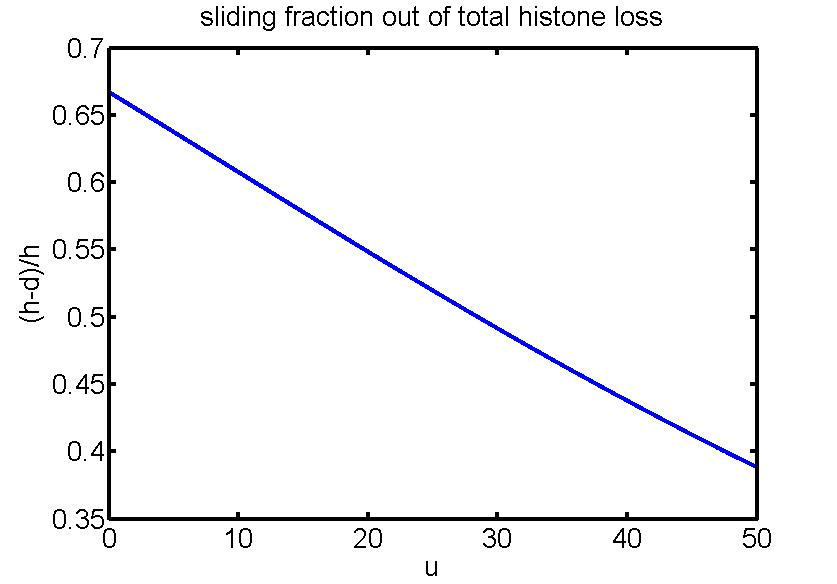
\includegraphics[width=0.5\linewidth, height=0.3\textheight]{Images/slidingFractionOutOfTotal}
\caption{}
\label{fig:slidingFractionOutOfTotal}
\end{figure}

The fraction of histone loss due to sliding out of the total number of histones in the ROI
\begin{equation}
\frac{1-g(u)}{\beta(u)}=(1-g(u))(1-d(u))
\end{equation}
Is shown in the figure below for uv dose 0 to 50 ms. exposure . 
\begin{figure}[H]
\centering
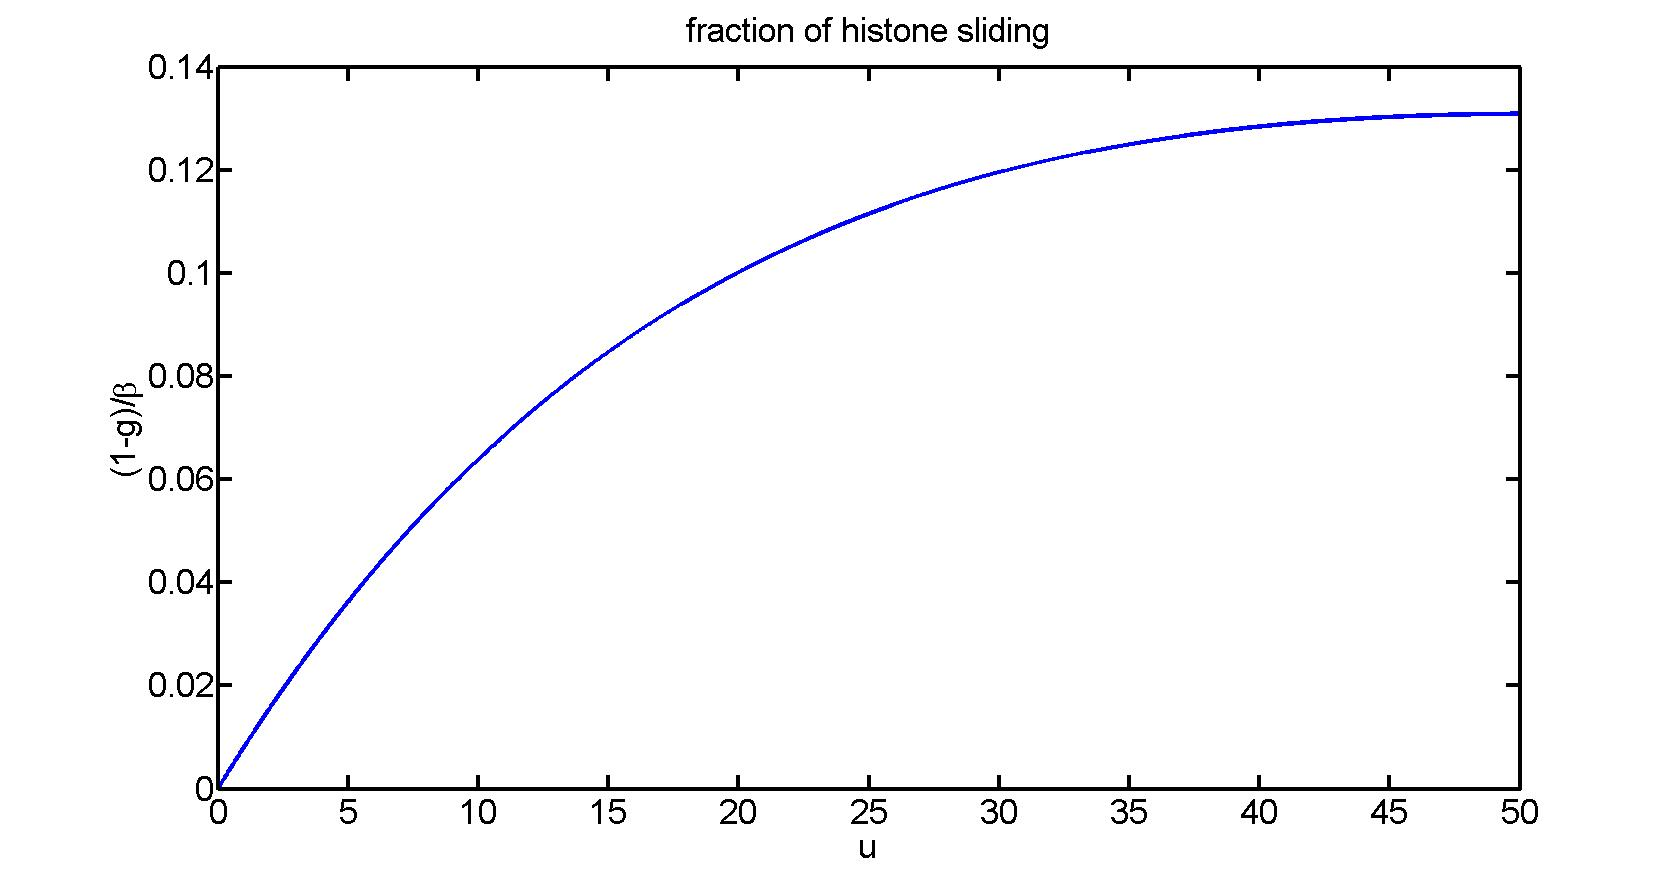
\includegraphics[width=0.7\linewidth, height=0.3\textheight]{Images/fractionOfHistoneSliding}
\caption{}
\label{fig:fractionOfHistoneSliding}
\end{figure}

\end{document}